\documentclass[letterpaper,notitlepage,twoside]{article}

% Basic imports, increase margins...
\usepackage[margin=0.75in]{geometry}
% Finite State Machine stuff
\usepackage{pgf}
\usepackage{tikz}
\usetikzlibrary{arrows, automata}
% Format tables nicely
\usepackage[latin1]{inputenc}
\usepackage{array}

\usepackage{amsfonts}
\usepackage{amssymb}
\usepackage{amsmath,amsthm}

\renewcommand{\implies}{\Rightarrow} % redefine command "implies"
\renewcommand{\iff}{\Leftrightarrow} % double arrow
\newcommand{\maps}{\rightarrow} % define command "map"
\newcommand{\union}{\cup}
\newcommand{\intersect}{\cap}
\newcommand{\N}{\mathbb{N}} % natural number
\newcommand{\Q}{\mathbb{Q}} % rational number
\newcommand{\R}{\mathbb{R}} % real number
\newcommand{\Z}{\mathbb{Z}} % integers
\newcommand\tab[1][1cm]{\hspace*{#1}} %\tab command

% Add more packages that you use here...

\begin{document}
\title{Homework 25}
\author{Brian Knotten, Brett Schreiber, Brian Falkenstein}
\maketitle
\subsection*{21}
Define the problem described as VDP (vertex disjoint paths). In order to show that $3SAT \geq _{poly} VDP$, we will first show that $VDP$ is self reducible. That is, given the decision problem for VDP, we can determine the paths connecting each $(s_i, t_i)$. \\\\
$VDP_{opt} \geq _{poly} VDP_{decision}$\\\\
Given as input to $VDP_{opt}$ a graph $G$ and a set of tuples $(s_1, t_1) ... (s_n, t_n)$, we can use the decision problem $VDP_{decision}$ to get the actual paths from each $s_i$ to each $t_i$. Define $P_i$ to be the path connecting $s_i$ to $t_i$. \\
First check if $VDP_{decision}$ on $G$ and $(s_1, t_1) ... (s_n, t_n)$ returns 1. If not, then paths don't exist. If 1, use breadth first search to get all neighbors of $s_1$, call these $v_1...v_k$. Now, call $VDP_{decision}$ on $G$ and $(v_i, t_1) ... (s_n, t_n)$ for $1\leq i \leq k$. If this returns 1, add $v_i$ to the path for $(s_1, t_1)$ $P_1$ and continue this process, searching for neighbors of $v_i$, etc. \\
Note that for each vertex added to a path $P_i$, we must make sure that that vertex does not appear in any other paths. We can enforce this by adding a new tuple to the input. If $v_i$ was the vertex added to the path for some $(s_i, t_i)$, then construct a new $(s, t)$ to be $(v_i, v_i)$. Since the shortest path from $v_i$ to $v_i$, it will always be an option to have its path be just $v_i$. This forces other subsequent paths to not include $v_i$. If we continue this process for all $k$ tuples, we will have the paths for all the inputs. \\
This transformation is poly time. For each tuple, we must perform BFS to get from $s_i$ to $t_i$, making one call to $VDP_{decision}$ at each point. Since BFS takes polynomial time in the number of vertices and edges in a graph ($O(|V| + |E|)$, in the worst chase, as all vertices and edges will be visited), and the number of edges is bound by the number of vertices (max E = $V^2$), if we say the number of vertices is $n$, than the time for each tuple will be $O(n^2)$. Doing this for all $k$ tuples gives us $(O(kn^2))$, where $k$ can be no larger than $n/2$ (pigeonhole principle, since we cannot repeat vertices, if each vertex in $G$ were assigned to either a source or a sink). Thus, if a polynomial time algorithm exists for $VDP_{decision}$, than one exists for $VDP_{opt}$. \\\\
$3SAT \geq _{poly} VDP_{opt}$\\\\
Since we have shown that $VDP_{opt} \geq _{poly} VDP_{decision}$, if we have a poly-time algorithm for $VDP_{opt}$, than we also have a poly-time algorithm for 3SAT (IE, if we assume we have a polynomial time algorithm for decision, than we have one for opt). \\
We will show how to construct an instance of VDP from an instance of 3SAT, such that the VDP instance is true if and only if the 3SAT instance is satisfiable. To model choosing a variable $x$ in 3SAT as either true or false, construct the following sub-graph: \\
$$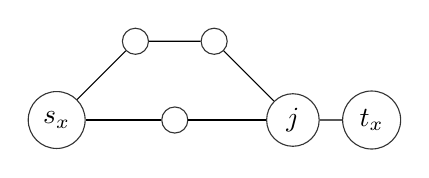
\begin{tikzpicture}
    \node[circle,draw=black!80] (a) at (0, 1) {$s_x$};
    \node[circle,draw=black!80] (b) at (1, 2) {};
    \node[circle,draw=black!80] (c) at (2, 2) {};
    \node[circle,draw=black!80] (d) at (1.5, 1) {};
    \node[circle,draw=black!80] (e) at (3, 1) {$j$};
    \node[circle,draw=black!80] (f) at (4, 1) {$t_x$};
    \draw (a) -- (b) -- (c) -- (e) -- (f);
    \draw (a) -- (d) -- (e);
\end{tikzpicture}$$
Here, there are 2 possible paths from $s_x$ to $t_x$, one of length 3 and one of length 4. Due to node $j$ being a bottleneck, only one of these paths can exist in the final output (as $j$ must be a member of both paths, they could not be disjoint). Take the path of length 3 being chosen to mean set $x$ to true, and the path of length $4$ being chosen to mean setting $x$ to false (or, setting $\overline x$ to true). Construct one such subgraph for each variable in the 3SAT instance. \\
Now, we must model the clauses in the 3SAT instance. That is, if the 3SAT formula is satisfiable, we will construct a subgraph that asserts that at least one of the literals in that clause will be true. 

\end{document}
